% !TeX root = ../my_thesis.tex
% !TeX spellcheck = en_GB
%!TEX TS-program = xelatex
%!BIB TS-program = biber

\chapter{Thermal Analysis of Natural Fibre Composites}\label{chap:p3}

\section*{Statement of Contribution}
	This chapter includes a co-authored book chapter. The bibliographic details of the published chapter are:
\begin{itemize}
	\item Javanbakht, Z, Hall, W \& Öchsner, A (2017), “Computational Evaluation of Transverse Thermal Conductivity of Natural Fiber Composites”, In: Improved Performance of Materials. Ed. by A Öchsner \& H Altenbach. Vol. 72. Advanced structured materials, Cham: Springer, pp. 197–206.
\end{itemize}
	My contribution as the corresponding author to the paper involved: undertaking literature review, classifying the necessary theoretical backgrounds and models, developing the programming code, analysing and discussing the finite element results, drawing figures, preparing tables, writing and editing the manuscript according to my supervisors’ comments.
	
\vspace{-0.5cm}
\Zia\\
\Wayne\\
\vfill
\newpage


\paragraph{Title:} Computational Evaluation of Transverse Thermal Conductivity of Natural Fiber Composites


\paragraph{Abstract.}The finite element analysis is used to investigate the sensitivity of the effective transverse thermal conductivity of polymeric composites reinforced with Manila hemp fibres in terms of their degree of saturation. It is predicted that the hierarchical structure of the fibre bundle will highly magnify the rate of water absorption and in consequence, the effective transverse thermal conductivity of the composite is altered. This influence is quantized in terms of the volume fraction of the fibre bundle and the lumen to produce a homogenized representative continuum. It was found that increasing the fibre volume fraction in a dry medium results in a decrease in the thermal conductivity whereas an increase of conductivity will be evident in a wet condition. Furthermore, the increase in the volume fraction of the lumen enhances the thermal conductivity by retaining more water during saturation which supports the developed hypothesis.

\section{Introduction}
	Natural fibres are widely used in various polymeric media for their typical low density, moderate cost, good specific strength, abundance and renewability of resources, and biodegradability among other favoured qualities. Nevertheless, the natural variability of properties, deficient fibre-to-matrix bonding, and more importantly their hydrophilic character introduce some challenges to their application. For instance, outdoor usage of natural composites is limited because of the susceptibility of their fibre reinforcements to environmental factors~\autocite{Assarar.2011,Placet.2009}.

	The porous structure of natural fibres makes them better thermal insulators compared to synthetic fibres such as glass or carbon~\autocite{Liu.2012}. On the other hand, their relatively low thermal conductivity may cause heat dissipation difficulties in some cases~\autocite{Kalaprasad.2000}. This trade-off attracted researchers in the past decades to investigate the naturally anisotropic thermal behaviour of these composites in terms of their volumetric composition~\autocite{Shah.2016}, volume fraction of fibres~\autocite{Li.2008}, fibre orientation~\autocite{Behzad.2007}, and thermal diffusivity~\autocite{Mangal.2003,Kalaprasad.2000} among other effective parameters.

	The mechanical properties of cellulose fibres are sensitive to the moisture content, particularly when incorporated into polymeric resins~\autocite{Faruk.2012}. Namely, the hygroscopic behaviour of natural fibres results in dimensional instabilities, i.e., swelling and shrinkage, which may induce residual stresses and microcracks into the composite as well as the debonding of the fibres~\autocite{Rakovsky.2014,Celino.2014}. From a macroscopic point of view, moisture initiates the degradation process of the natural fibres which in consequence, affects the properties of the composite. For instance, reduction of the elastic modulus and tensile strength~\autocite{Chow.2007,DHAKAL.2007}, fluctuation of the impact strength~\autocite{Athijayamani.2009}, and even the initiation of a fungal decay process~\autocite{Schirp.2007} is foreseeable. Herein, considering the porosity of the fibrous structure, it is hypothesised that the thermal conductivity of natural fibres is to be affected by the presence of water.
	
	Various theoretical and experimental methods were used to predict the thermal behaviour of natural fibres but the scarcity of the research on the effect of saturation motivated the current work, which is basically a computational effort to envision the big picture of the saturation process. In the current study, the effect of water content on the insulation role of a composite---reinforced with Manila hemp fibres in a high density polyethylene matrix---is investigated using the finite element method. A list of the used symbols in the current work is also provided, see Table~\ref{table:symbols4}.
\begin{table}[!h]
\centering
\caption{List of symbols}\label{table:symbols4}
\begin{tabular}{>{\centering}p{0.08\textwidth}p{0.78\textwidth}}
\toprule
$\gamma$ & mesh density\\
%$\zeta$ & volume fraction\\
$\zeta_{\text{f}}$ & volume fraction of the fibre bundle \red (volume of the solid part relative to that of the composite) \bl\\
$\zeta_{\text{l}}$ & volume fraction of the lumen \red (volume of the voids relative to that of the fibre bundle) \bl\\
$\mupDelta T$ &prescribed temperature gradient\\
$\ell$ & element edge length\\
$k_{\text{eff}}$ & effective thermal conductivity of the composite\\
$w$ &width of the RVE (the distance between the boundary faces)\\
$A_0$ &cross-sectional area perpendicular to direction of the flux\\
$\dot{Q}$ & total heat flux\\
$S_{\text w}$ &degree of saturation \\
$V_{\text f}$ & volume of the fibre bundle\\
$V_{\text{l}}$ & volume of the lumen (total voids) \\ 
$V_{\text w}$ & volume of the water\\
\bottomrule
\end{tabular}
\end{table}%


\begin{figure}[!b]
\centering
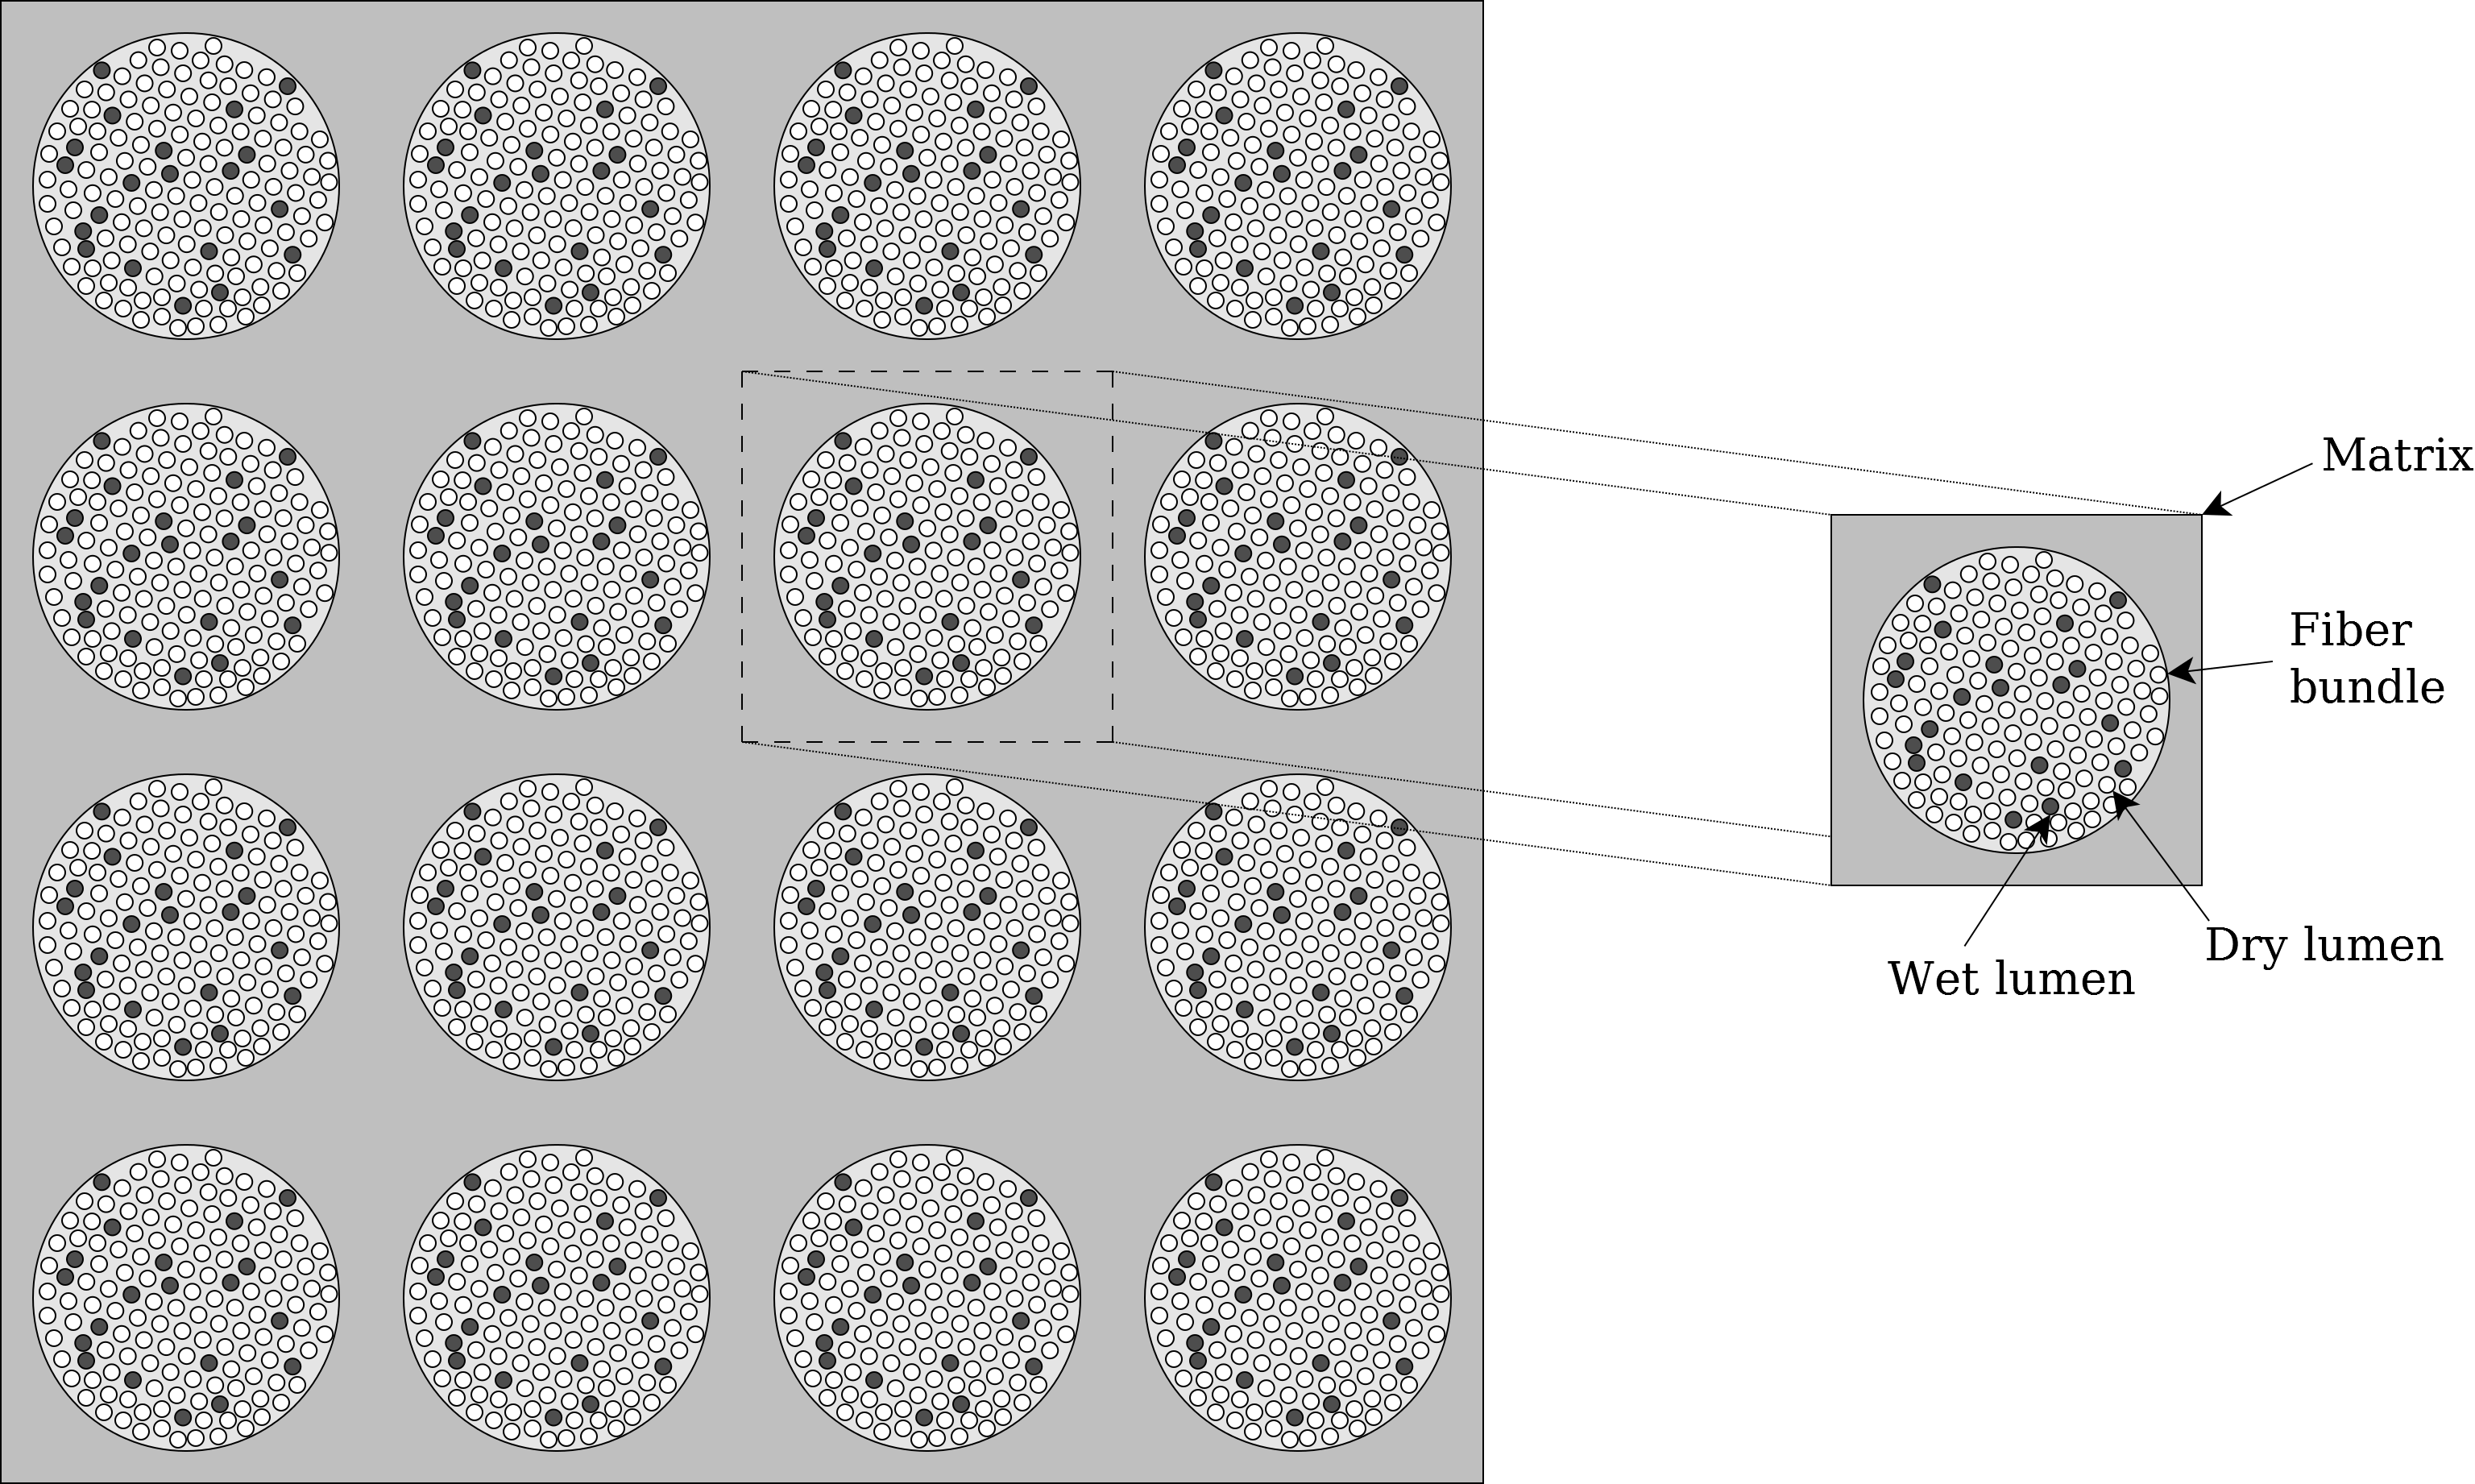
\includegraphics[width=\textwidth]{rve_heat}
\caption{Selected RVE from the unidirectional composite}\label{fig:rve}
\end{figure}


\red
\section{Composition of Natural Composites}
	\paragraph{Structure of hemp fibre composites} The composite is assumed to be made up of unidirectional hemp fibre bundles within a polymeric composite, see Fig.~\ref{fig:rve}. Each fibre bundle consists of a set of lumens, which are basically slender tubular structures that provide the air cavities~\autocite{Wang.2016}. Since the porosity of a natural fibre defines its capacity to hold water~\autocite{Rakovsky.2014}, the storage of moisture is done by filling the tubes with water and creating a wet lumen. Since no porosity is included in other components of the composite, lumens represent the total capacity of the fibre bundle to retain moisture. Dry lumens therefore provide the porosity whereas the remaining wet lumens hold the water in the composite.

\begin{figure}[!h]
\centering
\includegraphics[width=0.8\textwidth]{homo}
\caption{Homogenization process of the RVE}\label{fig:homo}
\end{figure}

	\paragraph{Components of the composite} A recent research shows that the bulk property of the fibrous structure can be properly modelled, within an acceptable margin of error, irrespective of the exact micro-level structure~\autocite{Liu.2011}. Therefore, a unit cell of the composite is selected as the RVE of the whole composite. In order to capture the hierarchy of the structure, the accumulated effect of the individual sub-structures are considered in four distinct layers: 
	\begin{enumerate}
	\item a polymeric matrix of high-density polyethylene (HDPE),
	\item the solid part of the Manila hemp fibre bundle,
	\item the water contained in the lumens, and
	\item the air which fills the remaining volume of the lumens.
	\end{enumerate}
	These four phases take part in the occurring thermal conduction process within the composite. The third phase vanishes in a 100\% dry fibre whereas the fourth phase is not available in completely saturated fibres.
	
	The thermal conductivities of the individual components of the composite are listed in Table~\ref{table:mat4}. This implies the fact that since the encapsulated water is stationary, no convection is taking place and the only means of heat transfer is the conduction mechanism~\autocite{Rakovsky.2014}.
	
\begin{table}[!bh]
\centering
\caption{Thermal conductivity of the composite components}\label{table:mat4}
\small
\begin{tabular}{p{0.2\textwidth}p{0.15\textwidth}p{0.4\textwidth}}
\toprule
\bfs{Component}&
\bfs{Material}&
\bfs{Conductivity} ($\scriptscriptstyle\frac{\text{W}}{\text{m}\cdot\text{K}}$)\\
\toprule
Matrix&
HDPE&
0.4025~\autocite{Rauwendaal.2014}\\
Solid fibre&
Hemp&
0.1847~\autocite{Liu.2011}\\
Lumen&
Air&
0.0026~\autocite{Liu.2011}\\
Moisture&
Water&
0.606~\autocite{Singh.2014}\\
\bottomrule
\end{tabular}
\end{table}	

	Finally, in the current study, the assumptions can be summarised into the following points:
	\begin{itemize}
		\item the porosity of the matrix and the solid portion of the hemp fibre bundle is neglected,
		\item all the porosity is provided by the lumens,
		\item the effect of the thermal barrier resistance is neglected,
		\item it is assumed that the thermal conductivity of the solid portion of hemp fibre bundles is independent of the lumen size,
		\item each component is assumed to be isotropic, and
		\item the thermal conductivity of all the components is assumed to remain constant by increasing the temperature.
	\end{itemize}
	As per these assumption, the following volume fractions can be defined:
	\begin{subequations}
	\begin{align}
	\zeta_{\text{f}}	&=\frac{V_{\text f}}{V_{\text c}},\\
	\zeta_{\text{l}}	&=\frac{V_{\text l}}{V_{\text f}},
	\end{align}
	\end{subequations}
	where $V_{\text f}$ is the volume of the whole fibre bundle, $V_{\text c}$ is the volume of the composite, $V_{\text l}$ is volume of the lumen, $\zeta_{\text{f}}$ is the volume fraction of the fibre bundle, $\zeta_{\text{l}}$ is the volume fraction of the lumen (relative to the volume of the fibre bundle). It is worth mentioning that the volume of the fibre bundle includes the solid volume plus dry and wet lumens. Namely, the fibre volume fraction is not only the fraction of the solid in the matrix.


	To represent the water content of the specimens, the degree of saturation~($S_{\text w}$) was used, which can be defined as follows:
\begin{equation}
S_{\text w}=\frac{V_{\text w}}{V_{\text{l}}},
\end{equation}
	where $V_{\text w}$ is the volume of the water, and $V_{\text{l}}$ is the volume of the lumen, which is equal to the total volume of the voids.
	




\red
\section{Micromechanical Model}
	Homogenisation of the continuous fibre-reinforced composites can be done by selecting a cylindrical RVE---which results in the so-called composite cylinder assemblage (CCA). This micromechanical model was first introduced in~\parencite{Hashin.1964} for evaluating the effective mechanical properties of hollow fibres within a matrix; the model is also called the composite spheres assemblage (CSA) and it is a two-phase model, i.e., a self-consistent model, which needs $n$-phase models for the same number of phases. Later, the mechanical properties of two-phase composite materials were considered in~\parencite{Christensen.1979} in a three-phase model. The latter effort marks the initial steps of the generalised self-consistent approach~\parencite{Bohm.2020} in which $n$-phase materials are modelled using $(n+1)$-phase models~\parencite{Herve.1993}. 
	
	By using several concentric cylinders in the CCA, each outer phase is modelled as a ring and the inner phase would be of a circular cross-section. Namely, the continuous fibres are replaced by a representative cross-section that implies the plain strain state for the problem. The homogenised medium would be of a circular cross-section that should admit to the boundary conditions of the original assembly. For instance in a thermal problem, two representations are linked together by enforcing the same temperature and heat flow on each of their boundaries. Originally, electrical conductivity of a two-phase composites was obtained in~\autocite{Kerner.1956b}. The same results of magnetic permeability of composite materials was obtained in~\autocite{Hashin.1962b} by means of variational principles. Later on, the interpretation of the latter resulted in the Hashin-Shtrikman bounds. 
	
	Herein, the CSA variant of the CCA model is adopted and extended to a four-phase composite in the context of thermal conductivity analysis. The CSA model was used to provide the benchmark values---the lower bound of the effective properties. It was shown that the differential equations of the CSA model (Fourier's transform law) could be used to incorporate additional phases in a spherical coordinate system~\autocite{Christensen.2012}. However, applying the continuity conditions on the interfaces and the boundary conditions on the outer surface creates a cumbersome process. By observing the repeating solutions of the differential equations in the middle rings, one could think of a recurring procedure. In~\parencite{Milton.2002}, such a procedure is introduced for particle-reinforced composites in which particle are covered with several coatings. By adopting several concentric spheres that represent each phase of four-phase natural fibre-reinforced composites, an analogous solution to the coated particles is readily obtained
	\begin{subequations}
	\begin{align}
		k_{\text{a-w}}     &= k_{\text{w}} + \frac{3(1-S_{\text{w}})k_{\text{w}}}{S_{\text{w}}-3\frac{k_{\text{w}}}{k_{\text{w}}-k_{\text{a}}}},\\\label{eq:airwater}
		k_{\text{a-w-f}}   &= k_{\text{f}} + \frac{3\zeta_{\text{l}}k_{\text{w}}}{1-\zeta_{\text{l}}-3\frac{k_{\text{f}}}{k_{\text{f}}-k_{\text{a-w}}}},\\
		k_{\text{a-w-f-m}} &= k_{\text{m}} + \frac{3\zeta_{\text{f}}k_{\text{w}}}{1-\zeta_{\text{f}}-3\frac{k_{\text{f}}}{k_{\text{f}}-k_{\text{a-w-f}}}},
	\end{align}
	\end{subequations}
	where `a', `w', `f', and `m' subscripts stand for air, water, fibre, and matrix, respectively. Thus, the effective thermal conductivity that results from the homogenisation of the air and water phases is denoted by $k_{\text{a-w}}$; a similar notation is used for the other two combinations. The four-phase micromechanical model can be readily solved by consecutive use of the CCA model for three times. By taking advantage of this approach, the $n$-phase model could be solved by $n-1$ equations/models.

\bl
\section{Methodology}
In the current study, the finite element method~\autocite{Ochsner.2013,Oechsner.2016} was used to estimate the effective thermal conductivity of unidirectional Manila hemp fibre bundles in the transverse (i.e., perpendicular to the principal fibre axis) direction. A four-phase continuum was created using the MSC.Marc (version 2014.2) commercial finite element package. This software was selected due to its capability of incorporating user-written pieces of code into its core algorithm. Namely, the customized procedures can be carried out using the subroutines written in the Fortran programming language~\autocite{Javanbakht.2017}. This facility---along with the provided Python scripting tool---makes it possible to fully automatize the parametric study~\autocite{Javanbakht.2016,Javanbakht.2016b}.

\red
	\paragraph{Mesh sensitivity} A 2D finite element model, with a thickness of the unit length, was created using a uniform mesh of elements of type 39, i.e., the 4-node bilinear isoparametric planar heat transfer elements. The uniform mesh density~($\gamma$) is defined using the following equation:
\begin{equation}
\gamma=\frac{1}{\ell_\text{mesh}},
\end{equation}
	where $\ell_\text{mesh}$ is the characteristic dimension of the element, i.e., the edge length of each square element. The used prototype for sensitivity analysis had a fibre volume fraction of 50\%, the typical lumen volume fraction of 30.87\%, and a water content of 25\%. Following several sensitivity analyses, a fluctuating of results was observed by refining the mesh. However, the mesh sensitivity was diminished for mesh densities over 300 and thus, a mesh density of 400 is used in the simulations, see Fig.~\ref{fig:sensitivty_hc1}. It is worth mentioning that the fibre overlap was allowed in all the simulation.

\begin{figure}[!h]{}
  \centering
	\includegraphics[scale=1]{hc1_mesh_sens}
  \caption{Sensitivity analysis of apparent thermal conductivity versus mesh density}
  \label{fig:sensitivty_hc1}
\end{figure}
\bl
	
	It is worth emphasizing that only one type of element was used with four different material properties, which represented the four distinct phases of the problem. Based on the volume fraction values of the fibre bundle and lumen plus the degree of saturation of the fibre, the occupied volume of each phase was calculated at the beginning of each analysis. In the next step, different properties were assigned to the elements by means of the \code{ANKOND} user subroutine. This subroutine is responsible for the anisotropic thermal behaviour of the material and it is called during the material assignments of the finite element analyses.
	
	Inasmuch as the prescribed temperature boundary conditions provide the most precise results in thermal conductivity analyses~\autocite{Islam.1999}, two set of prescribed temperatures were assigned to the left- and right-hand nodes of the RVE. Namely, a high temperature of $20^\circ\text{C}$ and a lower temperature of $0^\circ\text{C}$ were assigned as the boundary conditions. This established a temperature gradient, which was followed by a heat flux in the transverse direction, see Fig.~\ref{fig:sample}. The reaction heat flux of the lower temperature region was summed up and used to calculate the effective transverse thermal conductivity of the composite by means of Fourier's law~\autocite{Fiedler.2009}:
\begin{equation}
k_{\text{eff}}=\frac{\dot{Q}}{A_0}\cdot\frac{w}{\mupDelta T},
\end{equation}
	where $k_{\text{eff}}$ is the effective thermal conductivity of the composite, $\dot{Q}$ is the total reaction flux in the top boundary conditions, $A_0$ is the cross-sectional area perpendicular to direction of the flux, $w$ is the width of the RVE (distance between the boundary faces), and $\mupDelta T$ is the prescribed temperature difference.
\begin{figure}[t]
\centering
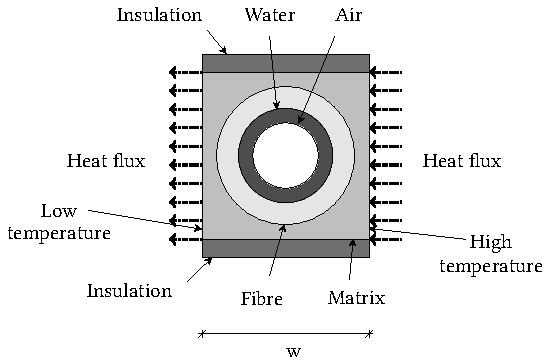
\includegraphics[width=0.6\textwidth]{chap4_fe}
\caption{Finite element model of the composite RVE}\label{fig:sample}
\end{figure}

\red
	\paragraph{Model validation} In order to validate the created prototype, the CSA model is used as the benchmark of the calculations. The typical value of 30.87\%~\autocite{Liu.2011} for the lumen volume fraction is taken along with the material properties listed in Table~\ref{table:mat4}. A range of fibre volume fraction from 10--50\% was taken to create Table~\ref{table:heat1_validation}; the effective thermal conductivity of the FE analyses and the CCA models are listed with the `RVE' and `CSA' subscripts, respectively. The percentage relative error ($e$) was calculated by deeming the CSA model as the benchmark. 

%\begin{table}[!h]
%\centering
%\caption{Simulation results of the mean thermal conductivity for various fibre volume fractions against the results of the CCA micromechanical model}\label{table:heat1_validation}
%\scriptsize
%\begin{tabular}{*{5}{P{0.06\textwidth}}}
%\toprule
%  \bfs{$\zeta_{\text{f}}$ (\%)}
%& \bfs{$S_{\text{w}}$ (\%)} 
%& \bfs{$k_\text{CCA}$} ($\scriptstyle\frac{\text{W}}{\text{m}\cdot\text{K}}$)
%& \bfs{$k_\text{RVE}$} ($\scriptstyle\frac{\text{W}}{\text{m}\cdot\text{K}}$)
%& \bfs{$e$ (\%)}
%\\
%\toprule
% 10 &0   &0.36542&	0.37984&	-3.95\\
% 10 &10  &0.36864&	0.38165&	-3.53\\
% 10 &20  &0.37157&	0.38338&	-3.18\\
% 10 &30  &0.37423&	0.38509&	-2.90\\
% 10 &40  &0.37667&	0.38652&	-2.62\\
% 10 &50  &0.37890&	0.38796&	-2.39\\
% 10 &60  &0.38096&	0.38936&	-2.20\\
% 10 &70  &0.38286&	0.39075&	-2.06\\
% 10 &80  &0.38463&	0.39194&	-1.90\\
% 10 &90  &0.38626&	0.39310&	-1.77\\
% 10 &100 &0.38779&	0.39427&	-1.67\\\midrule
% 20 & 0  &0.33054&	0.35845&	-8.44\\
% 20 &10  &0.33663&	0.36181&	-7.48\\
% 20 &20  &0.34218&	0.36523&	-6.74\\
% 20 &30  &0.34726&	0.36830&	-6.06\\
% 20 &40  &0.35192&	0.37109&	-5.45\\
% 20 &50  &0.35621&	0.37401&	-5.00\\
% 20 &60  &0.36018&	0.37670&	-4.59\\
% 20 &70  &0.36385&	0.37923&	-4.23\\
% 20 &80  &0.36727&	0.38167&	-3.92\\
% 20 &90  &0.37046&	0.38401&	-3.66\\
% 20 & 100&0.37344&	0.38624&	-3.43\\\midrule
% 30 & 0  &0.29768&	0.33813&	-13.59\\
% 30 &10  &0.30632&	0.34293&	-11.95\\
% 30 &20  &0.31423&	0.34772&	-10.66\\
% 30 &30  &0.32149&	0.35208&	-9.52\\
% 30 &40  &0.32818&	0.35637&	-8.59\\
% 30 &50  &0.33437&	0.36046&	-7.80\\
% 30 &60  &0.34011&	0.36426&	-7.10\\
% 30 &70  &0.34544&	0.36809&	-6.56\\
% 30 &80  &0.35042&	0.37162&	-6.05\\
% 30 &90  &0.35507&	0.37509&	-5.64\\
% 30 & 100&0.35942&	0.37831&	-5.25\\\midrule
% 40 & 0  &0.26668&	0.31873&	-19.52\\
% 40 &10  &0.27758&	0.32497&	-17.07\\
% 40 &20  &0.28760&	0.33101&	-15.09\\
% 40 &30  &0.29685&	0.33665&	-13.41\\
% 40 &40  &0.30540&	0.34221&	-12.05\\
% 40 &50  &0.31334&	0.34741&	-10.87\\
% 40 &60  &0.32072&	0.35249&	-9.91\\
% 40 &70  &0.32761&	0.35714&	-9.02\\
% 40 &80  &0.33404&	0.36186&	-8.33\\
% 40 &90  &0.34008&	0.36627&	-7.70\\
% 40 & 100&0.34574&	0.37054&	-7.17\\\midrule
% 50 & 0  &0.23736&	0.30036&	-26.54\\
% 50 &10  &0.25029&	0.30796&	-23.04\\
% 50 &20  &0.26222&	0.31504&	-20.15\\
% 50 &30  &0.27326&	0.32202&	-17.84\\
% 50 &40  &0.28352&	0.32854&	-15.88\\
% 50 &50  &0.29306&	0.33483&	-14.25\\
% 50 &60  &0.30198&	0.34092&	-12.90\\
% 50 &70  &0.31031&	0.34675&	-11.74\\
% 50 &80  &0.31813&	0.35239&	-10.77\\
% 50 &90  &0.32547&	0.35778&	-9.93\\
% 50 & 100&0.33237&	0.36302&	-9.22\\
% \bottomrule
%\end{tabular}
%\end{table}

\renewcommand{\arraystretch}{0.7}
\begin{table}[!h]
\centering
\caption{Simulation results of the mean thermal conductivity for various fibre volume fractions against the results of the CSA micromechanical model}\label{table:heat1_validation}
\small
\begin{tabular}{*{2}{P{0.08\textwidth}}*{2}{P{0.1\textwidth}}P{0.08\textwidth}}
\toprule
  \bfs{$\zeta_{\text{f}}$ (\%)}
& \bfs{$S_{\text{w}}$ (\%)} 
& \bfs{$k_\text{CSA}$} ($\scriptstyle\frac{\text{W}}{\text{m}\cdot\text{K}}$)
& \bfs{$k_\text{RVE}$} ($\scriptstyle\frac{\text{W}}{\text{m}\cdot\text{K}}$)
& \bfs{$e$ (\%)}
\\
\toprule
 10 &0   &0.36542&	0.37984&	-3.95\\
 10 &10  &0.36864&	0.38165&	-3.53\\
 10 &20  &0.37157&	0.38338&	-3.18\\
 10 &30  &0.37423&	0.38509&	-2.90\\
 10 &40  &0.37667&	0.38652&	-2.62\\
 10 &50  &0.37890&	0.38796&	-2.39\\
 10 &60  &0.38096&	0.38936&	-2.20\\
 10 &70  &0.38286&	0.39075&	-2.06\\
 10 &80  &0.38463&	0.39194&	-1.90\\
 10 &90  &0.38626&	0.39310&	-1.77\\
 10 &100 &0.38779&	0.39427&	-1.67\\\midrule
 20 & 0  &0.33054&	0.35845&	-8.44\\
 20 &10  &0.33663&	0.36181&	-7.48\\
 20 &20  &0.34218&	0.36523&	-6.74\\
 20 &30  &0.34726&	0.36830&	-6.06\\
 20 &40  &0.35192&	0.37109&	-5.45\\
 20 &50  &0.35621&	0.37401&	-5.00\\
 20 &60  &0.36018&	0.37670&	-4.59\\
 20 &70  &0.36385&	0.37923&	-4.23\\
 20 &80  &0.36727&	0.38167&	-3.92\\
 20 &90  &0.37046&	0.38401&	-3.66\\
 20 & 100&0.37344&	0.38624&	-3.43\\\midrule
 30 & 0  &0.29768&	0.33813&	-13.59\\
 30 &10  &0.30632&	0.34293&	-11.95\\
 30 &20  &0.31423&	0.34772&	-10.66\\
 30 &30  &0.32149&	0.35208&	-9.52\\
 30 &40  &0.32818&	0.35637&	-8.59\\
 30 &50  &0.33437&	0.36046&	-7.80\\
 30 &60  &0.34011&	0.36426&	-7.10\\
 30 &70  &0.34544&	0.36809&	-6.56\\
 30 &80  &0.35042&	0.37162&	-6.05\\
 30 &90  &0.35507&	0.37509&	-5.64\\
 30 & 100&0.35942&	0.37831&	-5.25\\\midrule
 40 & 0  &0.26668&	0.31873&	-19.52\\
 40 &10  &0.27758&	0.32497&	-17.07\\
 40 &20  &0.28760&	0.33101&	-15.09\\
 40 &30  &0.29685&	0.33665&	-13.41\\
 40 &40  &0.30540&	0.34221&	-12.05\\
 40 &50  &0.31334&	0.34741&	-10.87\\
 40 &60  &0.32072&	0.35249&	-9.91\\
 40 &70  &0.32761&	0.35714&	-9.02\\
 40 &80  &0.33404&	0.36186&	-8.33\\
 40 &90  &0.34008&	0.36627&	-7.70\\
 40 & 100&0.34574&	0.37054&	-7.17\\\midrule
 50 & 0  &0.23736&	0.30036&	-26.54\\
 50 &10  &0.25029&	0.30796&	-23.04\\
 50 &20  &0.26222&	0.31504&	-20.15\\
 50 &30  &0.27326&	0.32202&	-17.84\\
 50 &40  &0.28352&	0.32854&	-15.88\\
 50 &50  &0.29306&	0.33483&	-14.25\\
 50 &60  &0.30198&	0.34092&	-12.90\\
 50 &70  &0.31031&	0.34675&	-11.74\\
 50 &80  &0.31813&	0.35239&	-10.77\\
 50 &90  &0.32547&	0.35778&	-9.93\\
 50 & 100&0.33237&	0.36302&	-9.22\\
 \bottomrule
\end{tabular}
\end{table}
\renewcommand{\arraystretch}{1}
	
	It was observed that by increasing the fibre volume fraction, the relative error increases from a minimum of 1.77\% to a maximum of 26.54\%. The RVE seemed to slightly overestimate the effective thermal conductivity. Moreover, by increasing the water content, the FE values approach the values of the CSA model. Overall, the FE prototype showed an acceptable range of errors. Nevertheless, the results of the analyses with lower volume fractions seemed to be closer to the lower bound provided by the CSA model.
\afterpage{\clearpage}
\bl

\section{Results and Discussion}
	In a typical hemp fibre, the average diameter of the fibre bundle and lumens are 213 and 16.5 microns, respectively. Also an average number of 137 lumens exists in every fibre bundle, which results in an average lumen volume fraction of 30.87\%\,\footnote{\red Note that the calculation of average lumen fraction was carried out in this reference based on a histogram, and thus the reported average numbers will not results in the value of 30.87\%; see the reference~\autocite{Liu.2011} for further details.\bl}~\autocite{Liu.2011}. The saturation of this typical hemp fibre was simulated and the effective transverse thermal conductivity of the composite was calculated using the accumulated reaction heat fluxes, see Fig.~\ref{fig:typical}.
	
\begin{figure}[!h]
  \centering
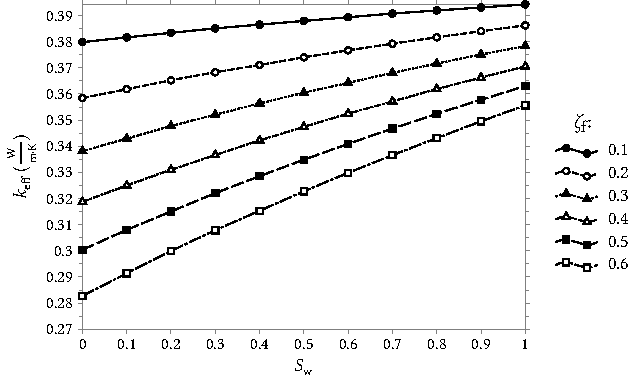
\includegraphics[scale=1]{typical}
  \caption{Effective transverse thermal conductivity of a typical lumen fraction ($\zeta_{\text{l}}=30.87\%$)}
  \label{fig:typical}
\end{figure}

	\red 
	As mentioned earlier, increasing the volume fraction adds to the amount of both the solid and lumen components. Therefore by increasing the fibre volume fraction, a completely dry fibre loses its thermal conductivity. This is due to the lower thermal conductivity of both fibre and air with respect to the matrix; thus, an isolation effect in dry fibre is expected. On the other hand, by increasing the fibre volume fraction in completely saturated fibres a milder isolation is obtained. This can be attributed to the thermal conductivity of water, which is higher than that of the matrix, and works in the opposite direction of fibre increase.\bl


	Furthermore in Fig.~\ref{fig:typical}, it can be noted that by increasing the degree of saturation, the effective thermal conductivity experiences an increase, which happens at a higher rate for the higher fibre bundle volume fractions. For instance, for a fibre bundle volume fraction of 60\%, the saturation causes an increase of the thermal conductivity by 25.79\% whereas the same value was only improved by 3.79\% for a volume fraction of 10\%. In other words, although the lumen fraction is kept constant, the amount of absorbed water increases due to the overall increase in the cross-sectional area of the fibre bundle.
	
	The effect of lumen volume fraction is investigated for two extreme fibre bundle volume fractions, i.e., a high volume fraction of 60\% and low volume fraction of 10\%, see Figs.~\ref{fig:low} and \ref{fig:high}. Increasing the lumen volume fraction in either case results in an increase in the effective thermal conductivity due to saturation. This effect is augmented at higher fibre bundle volume fractions. For example, the complete saturation of a low fibre content composite with a small lumen volume fraction increases the transverse thermal conductivity by only 1.24\% whereas a high content fibre with a high lumen volume fraction undergoes a 44.61\% improvement.

	
\begin{figure}[!h]{}
  \centering
 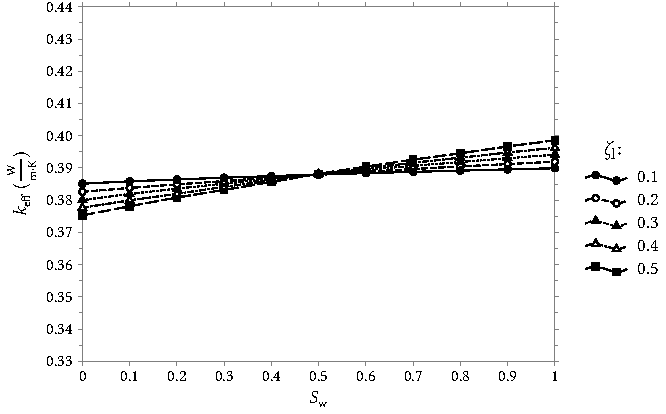
\includegraphics[scale=1]{low}
  \caption{Effective transverse thermal conductivity of low fibre volume fraction composite ($\zeta_{\text{f}}=10\%$)}
  \label{fig:low}
\end{figure}

\begin{figure}[!h]{}
  \centering
 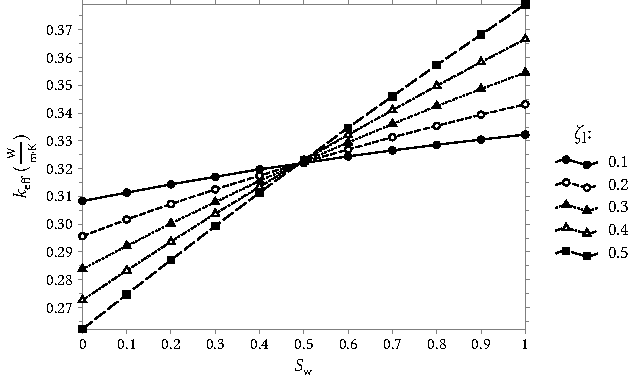
\includegraphics[scale=1]{high}
  \caption{Effective transverse thermal conductivity of high fibre volume fraction composite ($\zeta_{\text{f}}=60\%$)}
  \label{fig:high}
\end{figure}

\red
	One interesting point in both Figs.~\ref{fig:low} and \ref{fig:high} is the fact that around 50\% saturation, all lumen volume fractions result in the same apparent thermal conductivity. This could be justified by the setup of the FE model; the water component has a relatively high thermal conductivity and it surrounds the air phase in the middle, see Fig.~\ref{fig:sample}. It seems that the saturations around 50\% could redirect the heat flow around the air phase irrespective of the lumen volume fraction. From another point of view, by observing Eq.~\eqref{eq:airwater}, one could see that the contribution of the water-air phase depends only on the degree of saturation.\,\footnote{This statement implies that the thermal conductivities are assumed to be constant.} Nevertheless, this outcome requires further investigations, e.g., an experimental validation.
\bl

	In the dry composite samples, increasing the fibre bundle volume fraction reduces the effective thermal conductivity for a specific lumen volume fraction. Similarly, increasing the lumen volume fraction for a specific fibre bundle volume fraction, decreases the thermal conductivity of the specimen, see Fig.~\ref{fig:dry}. On the other hand, in a fully saturated composite sample, the effect is opposite to that of the dry sample due to the higher thermal conductivity of the absorbed water compared to air, see Fig.~\ref{fig:saturated}.
\begin{figure}[!h]{}
  \centering
 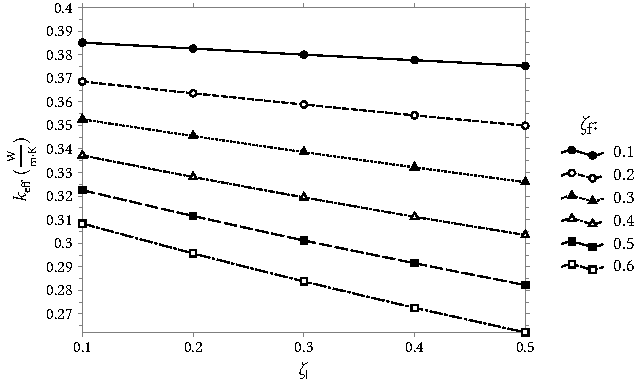
\includegraphics[scale=1]{dry}
  \caption{Effective transverse thermal conductivity of dry composite specimens}
  \label{fig:dry}
\end{figure}

\begin{figure}[!h]{}
  \centering
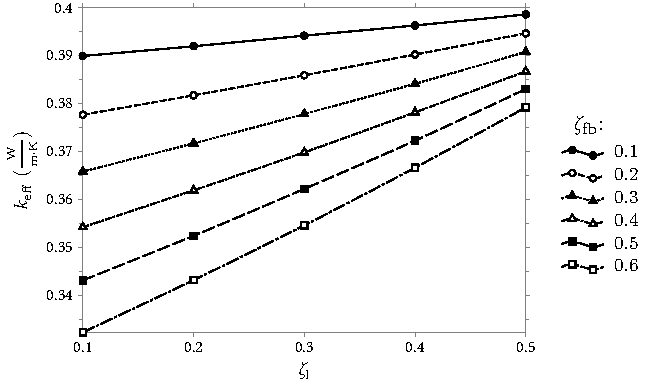
\includegraphics[scale=1]{sat}
  \caption{Effective transverse thermal conductivity of fully saturated composite specimens}
  \label{fig:saturated}
\end{figure}
\newpage
\section{Conclusion}
\red
	In summary, an FE model was introduced for evaluating the apparent/effective thermal conductivity of the Manila hemp fibres---this method, however, is applicable to every type of natural fibre composites. After validating the FE model with the composite spheres assemblage model, a typical case was analysed. It was shown that dry fibres have an isolation effect, which becomes more pronounced at higher fibre volume fractions. A milder isolation was observed for the fully saturated state.\bl\ It was shown the porosity of the Manila hemp fibre bundles affected the effective transverse thermal conductivity of the natural composite. Namely, by increasing the lumen fraction, a decrease was observed in the dry samples whereas an improvement happened in the effective thermal conductivity of the fully saturated samples. This effect was highly augmented in high fibre bundle volume fractions since the amount of water absorption was increased due to the increased volume of the voids within the fibre bundle. In consequence, the effective transverse thermal conductivity of the composite was increased. \red\ In future studies, carefully-controlled experimental studies should be conducted to refine the possible shortcomings of the FE model, e.g., the mesoscopic heat flow around 50\% saturation.\bl



